\chapter{编队控制飞行实验}%TODO:仿真需要给出控制器的相关参数,以及初始条件等等。
\label{chap:simulatin_expermient}
上一章介绍了无人机编队控制器的仿真环境,并基于MATLAB/Simulink
工具以及Gazebo仿真环境分别分别完成了数学仿真以及动力学仿真,验证了
前文所设计编队控制器的合理性。
本章中,则从双机编队的实物飞行实验的角度出发,介绍双机编队的软硬件
环境选配、硬件连接、通讯搭建等方面介绍固定翼无人机双机编队的硬件解决方案
以及飞行试验过程。
\section{无人机软硬件环境选配}
本文所设计的编队控制器是以开源自动驾驶仪PX4的内环为基础的,PX4的内环自动驾驶仪运行在Pixhawk这一开源硬件之上,成为上层控制的下位机(slave computer):
编队控制算法运行在具有ROS环境的上位机(host computer)中;
整体的软件硬件选配关系如下图所示:
\begin{figure}[H]
    \centering
    \includegraphics[width=1\textwidth]{figures/c4/c4-soft-hard.png}
    \caption{硬件软件选配关系}\label{fig:c4-soft-hard.png}
\end{figure}
上位机(host computer)的选择主要由其性能决定,应满足ROS基本环境的正常运行以及编队控制算法的需求;其次应考虑该硬件的寿命,体积,工况
要求等指标。下位机(slave computer)是PX4等算法运行的介质,也是飞行之中的重要传感器如惯性原件(IMU)、磁罗盘以及定位模块(GPS Module)的
工作平台,选择时考虑其传感器精度,平台计算能力等因素;无人机是编队控制的载具平台,应根据上述硬件以及必要航电设备选择翼面积、起飞质量
有效载荷等重要参数;根据硬件安放位置选择合适的机舱外形;根据编队控制需要确定平飞速度;根据期望推力选择发动机型号;根据起飞降落方式
选择起落架类型。必要时,应根据性能要求以及指标设计无人机。
\section{双机编队通讯连接}
在实现无人机编队过程中,双机通信必不可少。通信模块相对于无人机系统相对独立,在此只介绍硬件实现的一种手段:通讯模块选用P900芯片,通讯协议
选用mavlink协议,驱动由ROS下的串口功能包“serial”提供;领机将自身的状态信息通过串口从其自动驾驶仪滤波之后的值中获取
,之后进行mavlink的编码,最后通过数传模块发送之后,接收端进行解包;实际双机编队飞行试验的硬件链接逻辑如下图所示:
\begin{figure}[H]
    \centering
    \includegraphics[width=1\textwidth]{figures/c4/double_plane_real}
    \caption{双机编队通讯连接}\label{fig:c4-double_plane_real}
\end{figure}
双机编队时,领机的实时状态信息由Pixhawk飞控进行滤波之后得出,之后
通过串口通信方式,通过数据线被领机上位机读取;之后上位机对读取的领机状态消息进行
打包以及MAVlink协议编码,之后再调用相应的串口驱动功能包,驱动P900数传模块
进行发送。

从机端,上位机读取无人机状态信息的机制与领机相一致,除此之外,从机还需接收
来自领机数传模块中的领机状态信息,之后上位机再进行解包操作,获取
领航无人机的状态信息之后,按照前文介绍的编队控制的相关算法,最终产生
自驾仪内环的期望推力以及期望姿态角等信息,并通过串口通信的方式发送给
自动驾驶仪。

地面端,使用一个接收基站来接收来自两架无人机的回传信息,之后再通过WIFI
再将双机的飞行状态信息发送到地面站上,以做出相应的记录以及监视。另外,
通过地面站软件,还可以对领航无人机实行预先的航迹规划,并且可以在航迹
之中设计盘旋,拍照触发等相应的动作指令。进一步的,在实验的初期阶段
可通过运行QgroundControl地面站进行PX4自动驾驶仪的内环参数在线整定
工作,并对应相应的变化曲线,实时记录参数整定的相关过程,以及参数效果
对比等功能。
\section{双机编队实验安全保障机制}
本节的安全保障机制是出于对于实验人员以及实验设备的保护而特别
设计的,由于外场环境因素的不确定性以及硬件设备的不确定性,容易导致
初期实验时的无人机出现异常,因而设计相关的保护机制是十分有必要的。
\subsection{无人机飞行的地理围栏}
当实验基地周围有重要建筑或高危险领域需使无人机飞行时予以避让时,应使用
地理围栏保护机制。
所谓地理围栏,就是一种规划于无人机飞行任务中的虚拟屏障,一般由规则的
几何形状确定,如下图所示:
\begin{figure}[H]
    \centering
    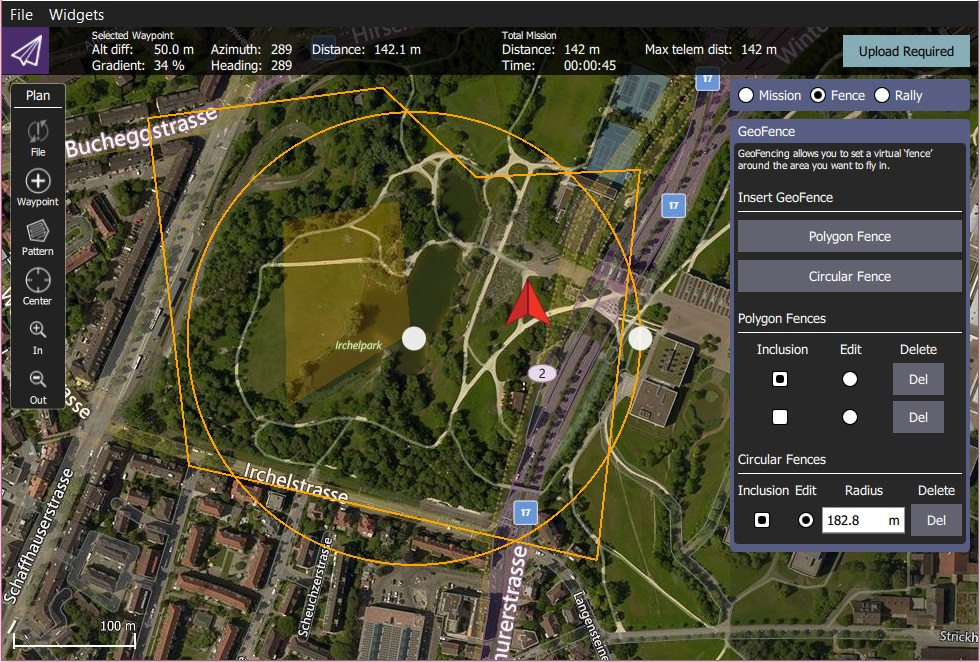
\includegraphics[width=0.85\textwidth]{figures/adds/geofence_overview}
    \caption{圆形以及多边形地理围栏示意图}\label{fig:c5-geofence_overview}
\end{figure}
当无人机因为异常飞越预先设置的地理围栏之后,会自动触发返航机制,随后
无人机将放弃当前所在执行的相关任务而进入返航模式。地理围栏机制在控制
的逻辑上高于自动任务模式和编队时所需的上位机外部控制模式,因而可以在
各种情况下进行保护。
\subsection{编队异常切出}
编队异常,主要的发生原因有二:第一,通讯失联导致领航无人机的状态信息
只有部分或者完全不能被从机接收到,此时,编队控制器运行时无法正确计算
出期望的内环输入,如果不加限制,就会出现控制异常的情况。第二,控制
器硬件出现问题,导致重要传感器数据不准确或者错误。例如:消费级别的
加速度计以及陀螺仪等惯性原件在受到撞击之后,容易出现姿态测量不准确
的情况;GPS定位模块在有些地理环境下可能会出现无法搜索定位卫星的情况,
导致位置测量不准确。上述硬件原因导致自动驾驶仪出现控制失效。
针对上述二种异常情况,对应的解决措施是:

第一种情况下,可设计一飞行监控节点,内部逻辑则是一个有限状态机,实时
判断接收消息的正确有效性。监控飞机当前的状态以及外部条件,控制飞机
进入不同的模式,并为异常模式设置如返航等保护方案。
\begin{figure}[H]
    \centering
    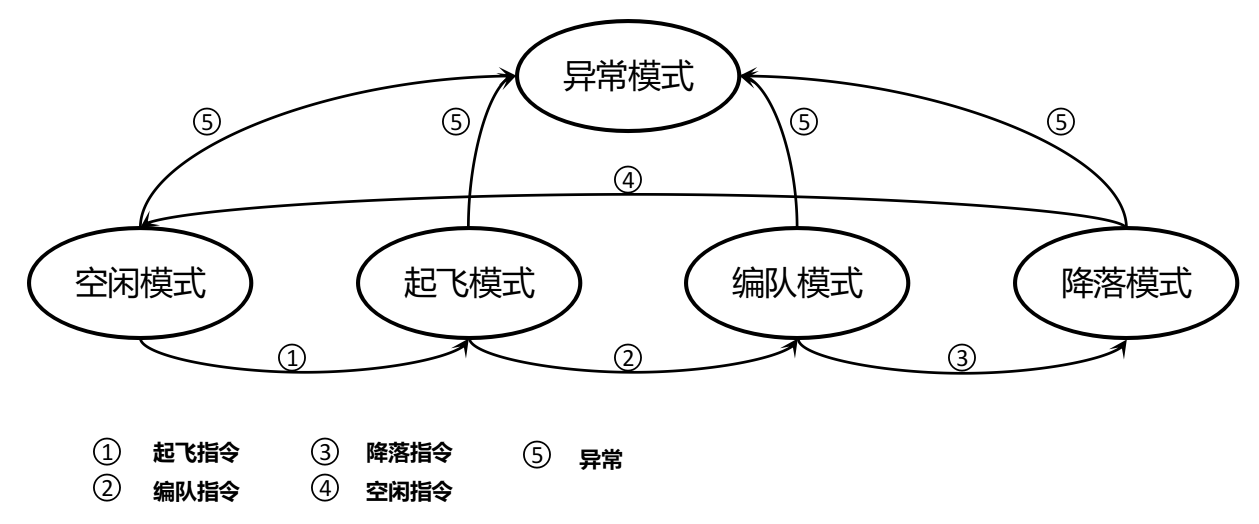
\includegraphics[width=0.85\textwidth]{figures/adds/states_mech}
    \caption{双机编队有限状态机逻辑示意图}\label{fig:c5-states_mech}
\end{figure}

针对情况二,此时自动驾驶仪硬件出现问题,应立刻放弃无人机的自主控制,
转而使用地面操纵员的手动飞行。在手动飞行模式下的通讯如下图所示:
\begin{figure}[H]
    \centering
    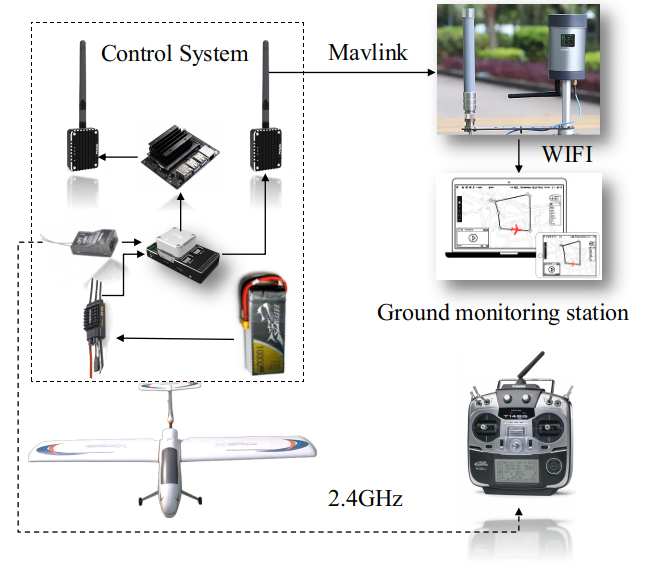
\includegraphics[width=0.85\textwidth]{figures/adds/protected_arch}
    \caption{手动飞行模式下的通讯连接}\label{fig:c5-protected_arch}
\end{figure}
手动飞行模式下,来自地面操纵员的指令信息直接由接收机接收,控制信号
直接通过Pixhawk,不经过任何处理直接接入飞机的四个控制通道。如此一
便可保证在操纵员的控制下迫降无人机。
\section{双机编队实验方案设计}
本文在设计双无人机编队飞行试验时,按照从“子系统到完整系统”的原则将
完整的双机飞行实验分为三部分:
\begin{enumerate}
    \item 分系统实验:\\
        本部分主要关注无人机分系统的可靠性。首先进行通讯模块测试:
        将通讯模块与上位机相连接,为测试编写实验性程序,分别测试
        点对点通讯模式、点对多点通信模式以及多点对多点组网通信模式;
        之后选取不同的通讯距离,例如0.5km、1.0km和1.5km等间距点,测试
        通讯模块在不同条件下的丢包率,并根据合理的通讯范围设计后续实验
        的航迹路径。之后,对自动驾驶仪传感器进行测试以及校准:进行无人
        的地面实验,着重测试风速计、气压计、加速度计和陀螺仪等惯性原件
        以及GPS定位模块的精度、噪声等相关指标。
    \item 硬件在环实验:\\
        此处的硬件在环指的是领机以及从机的各个分系统分别作为仿真环节参与整个编队
        控制的实验。编队的硬件在环实验的逻辑关系如下图所示:
        \begin{figure}[H]
            \centering
            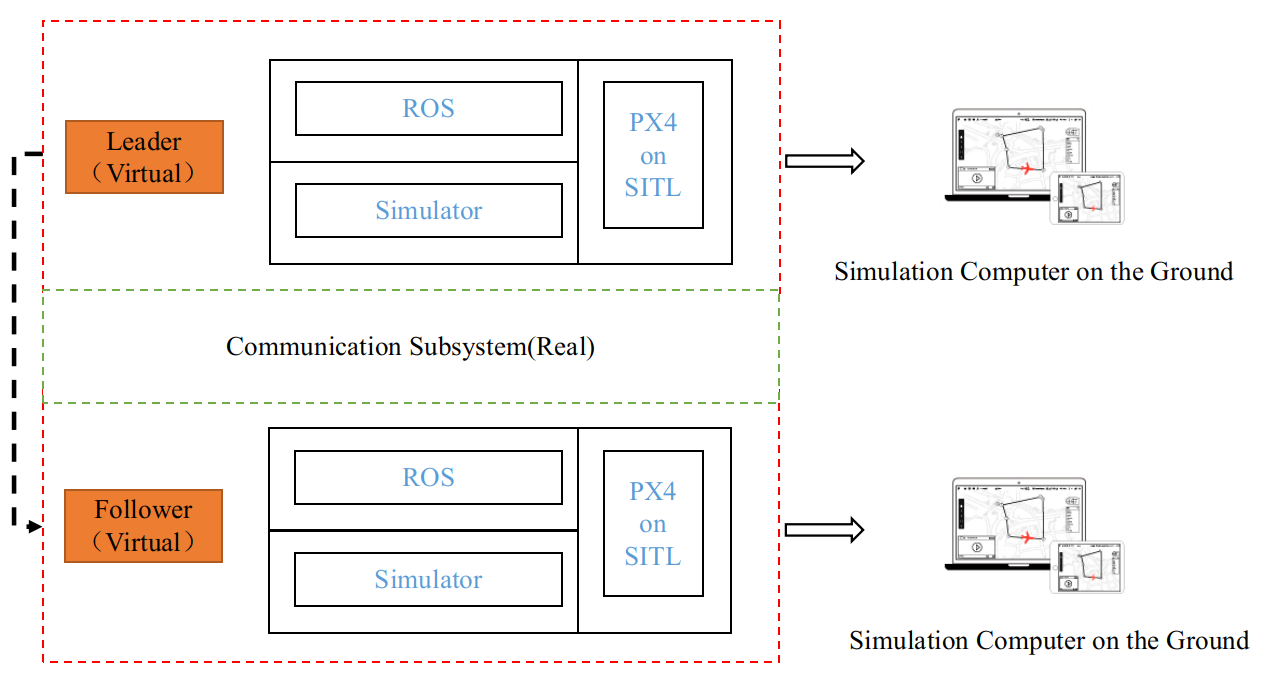
\includegraphics[width=0.85\textwidth]{figures/adds/hard_loop_com}
            \caption{通信子系统硬件在环实验逻辑图}\label{fig:hard_loop_com}
        \end{figure}
        \begin{figure}[H]
            \centering
            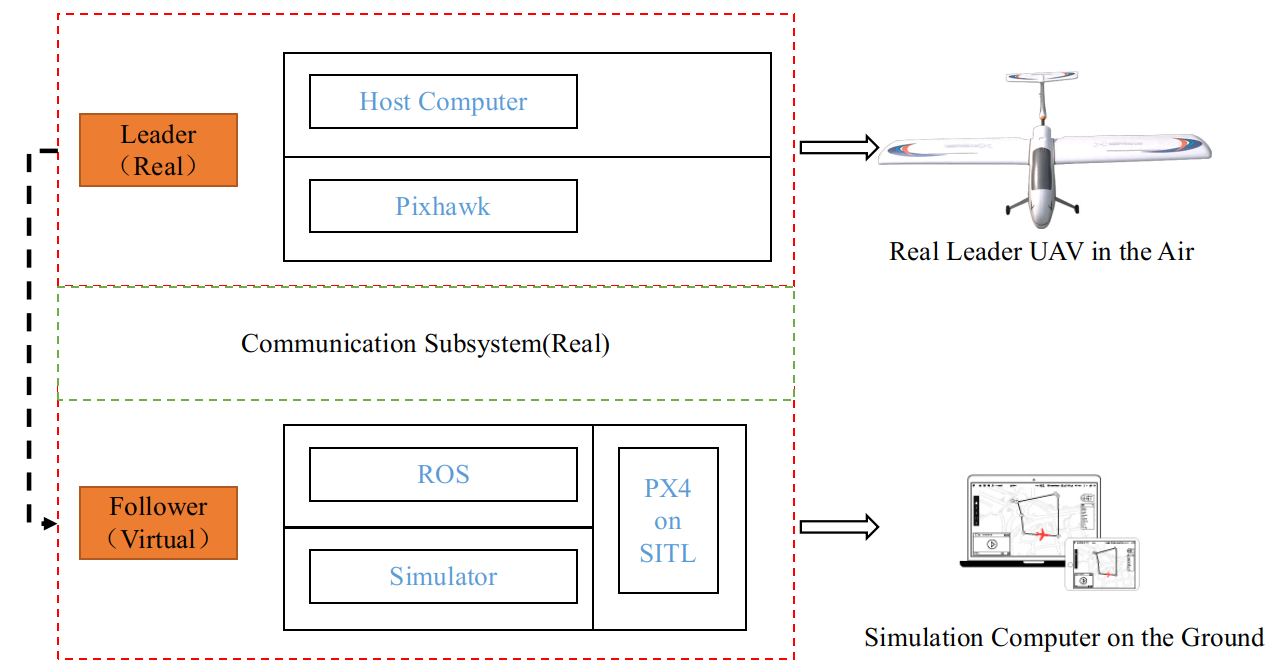
\includegraphics[width=0.85\textwidth]{figures/adds/hard_loop_leader}
            \caption{领航无人机硬件在环实验逻辑图}\label{fig:hard_loop_leader}
        \end{figure}
        \begin{figure}[H]
            \centering
            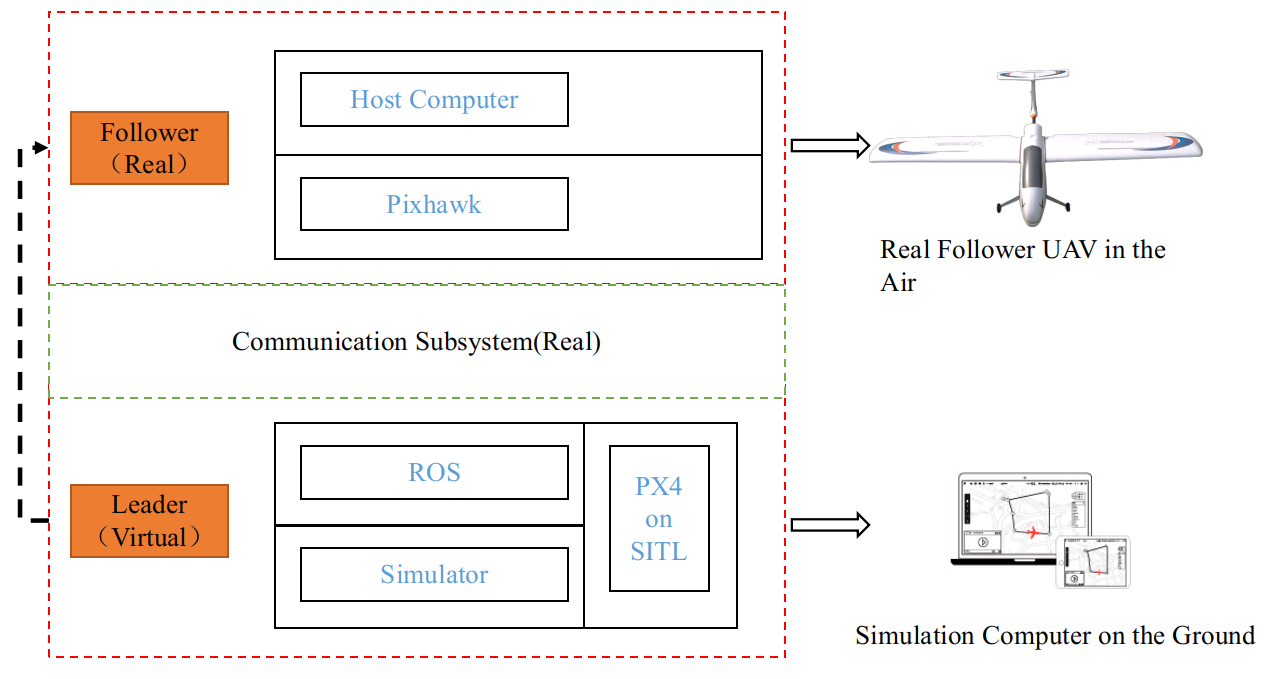
\includegraphics[width=0.85\textwidth]{figures/adds/hard_loop_fol}
            \caption{跟随无人机硬件在环实验逻辑图}\label{fig:hard_loop_fol}
        \end{figure}
        通过硬件在环实验,可以验证独立验证在真实飞行条件下的无人机各个子系统
        的实际工作情况,并可以在此阶段得到较为实际的编队控制器以及自动驾驶仪内环的
        参数整定情况。
    \item 完整系统飞行实验:\\
        在分系统实验、硬件在环实验完成之后,可进行完整系统的实验,首先
        按照第二部分实验整定完毕的控制器参数进行设定,使用地面站软件规划
        航线之后进行起飞,完成双机编队飞行实验。飞行实验之中,应
        结合数据记录工具进行实验数据的采集:本实验中,应记录:
        跟随无人机与期望位置的位置误差,与领机的速度误差随时间
        变化的关系。
        下图展示了使用本章中所介绍的控制器硬件进行无人机飞行编队的实验效果:
        \begin{figure}[H]
            \centering
            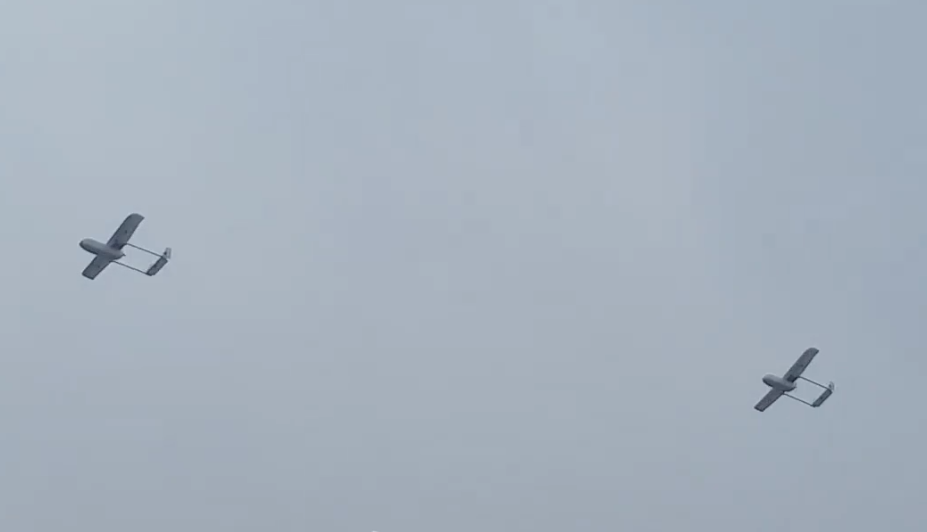
\includegraphics[width=0.85\textwidth]{figures/adds/real_test}
            \caption{硬件解决方案实际飞行效果}\label{fig:real_test}
        \end{figure}
        需要说明的是:上图中所展示硬件平台与本文中所介绍的在控制系统层面完全一
        致,固定翼无人机载具当时根据载荷的要求选取了另一有效载荷较小的无人机平
        台。另外本文的编队控制器是在上图飞行中所运用的控制器的改进版本。
\end{enumerate}
\section{本章小结}
本章主要介绍了编队控制实际飞行时的硬件平台的选择,介绍了无人机编队
控制使用的上位机、下位机以及无人机载具的相关配置。之后,按照所选用
编队控制硬件,设计了遵循”从子系统到完整系统“的相关实验,为今后进一
步进行实物实验提供了一种解决方案。
